\chapter{Experiments and Results}
\label{cha:experiments}

\section{Experimental Setup}
\label{sec:experimental-setup}

\begin{comment}
Trying and failing is a major part of research. However, to have a chance of success you need a plan driving the experimental research, just as you need a plan for your literature search. Further, plans are made to be revised and this revision ensures that any further decisions made are in line with the work already completed.

The plan should include what experiments or series of experiments are planned and what questions the individual or set of experiments aim to answer. Such questions should be connected to your research questions, so that in the evaluation of your results you can discuss the results wrt to the research questions.
\end{comment}

\begin{comment}
The experimental setup should include all data --- parameters, etc. --- that would allow a person to repeat your experiments.
This will thus be the actual instantiation for each experiment of the general architecture described in Chapter~\ref{cha:architecture}.
\end{comment}

The experiments conducted to evaluate the performance of GeoGPT on geospatial tasks are divided into two approaches. These are presented in \autoref{subsec:benchmarking-setup} and \autoref{subsec:prompt-quality-test-setup}.


\subsection{Quantitative Approach: Benchmarking}
\label{subsec:benchmarking-setup}

The first approach seeks to evaluate its ability to successfully answer questions that have a concrete answer. To do this, a Q\&A dataset was constructed. This dataset consists of set of 12 GIS-related questions with corresponding correct answers. For each record in the dataset, a description of how a human would find it natural to approach the problem. This description is provided as a step-by-step path towards the solution, and is only included to guide any reader as to how the system would be expected to solve the system. The full Q\&A dataset can be found in \autoref{tbl:questions-quantitative}. This set of experiments will allow for quantitative assessment of GeoGPT's GIS-abilities, and is a feasible way of benchmarking the system.

Another aspect that the benchmarking approach will try to evaluate is the consistency of the system, its ability to repeatedly provide an acceptable answer to the same user question. Each of the 12 questions are therefore asked three times per agent type.

With the implementation of three different agent types, the total number of test runs becomes the following: $$12 \text{ questions} \cdot 3 \text{ agent types} \cdot 3 \text{ repetitions} = 108 \text{ tests}$$


\subsubsection{Outcome Evaluation}

Each test run's answer will be manually evaluated, and the outcome will be annotated as one of \textit{success}, \textit{partial success}, and \textit{failure}. \autoref{tbl:test-outcome-enum} shows the guidelines used when assigning test results.

\begin{table}[htbp]
    \centering
    \caption{Description of Success}
    \label{tbl:test-outcome-enum}
    \begin{tabularx}{0.9\textwidth}{p{3cm}X}
        \toprule
        \textbf{Outcome} & \textbf{Guideline}                                                                                                                                                                                  \\
        \midrule
        Success          & The question was answered correctly and little to no follow-up from the user was required to produce the desired outcome. No false assumptions were made by the system when answering the question. \\
        Partial Success  & Portions of the question were answered correctly or semi-correctly, and/or some follow-up from the user was required to guide the system toward the solution.                                       \\
        Failure          & The question was answered incorrectly answered and/or false assumptions were made by the system while attempting to answer the question.                                                            \\
        \bottomrule
    \end{tabularx}
\end{table}

The annotated outcomes are then encoded using the ordinal encoding presented \autoref{tbl:outcome-encoding}. A higher value indicates a better outcome. These encoded outcome values enable standard deviation calculations, which serve as a suitable measure for assessing repeatability. This approach also allows for comparisons across different agent types and configurations.

\begin{table}[htbp]
    \centering
    \caption{Encoding for Test Outcome}
    \label{tbl:outcome-encoding}
    \begin{tabularx}{0.5\textwidth}{XX}
        \toprule
        \textbf{Outcome} & \textbf{Encoded Value} \\
        \midrule
        Success          & 2                      \\
        Partial Success  & 1                      \\
        Failure          & 0                      \\
        \bottomrule
    \end{tabularx}
\end{table}


\subsubsection{Other Metrics}

The application is hooked up to LangChain AI's tracing system, \textit{LangSmith}. Apart from being a useful tool for debugging purposes, it provides a simple way of obtaining detailed data for token and time usage for a particular run, as well as the total cost of the run. These are metrics that will be recorded and used in the evaluation of GeoGPT.

To summarize, the following metrics are recorded for a given test run:

\begin{itemize}
    \item The outcome of the test (\textit{success}, \textit{partial success}, or \textit{failure})
    \item The total duration in seconds
    \item The total number of tokens used
    \item The total cost for the run in American dollar
\end{itemize}


\begin{longtable}{p{4cm}p{4.5cm}p{4.5cm}}
\caption{Questions for GIS benchmark experiment} \label{tbl:questions-quantitative} \\
\toprule
\textbf{Query} \textbf{ID} & \textbf{Query} & \textbf{Correct} \textbf{Response} \\
\midrule
\endfirsthead
\caption[]{Questions for GIS benchmark experiment} \\
\toprule
\textbf{Query} \textbf{ID} & \textbf{Query} & \textbf{Correct} \textbf{Response} \\
\midrule
\endhead
\midrule
\multicolumn{3}{r}{Continued on next page} \\
\midrule
\endfoot
\bottomrule
\endlastfoot
aker\_brygge\_national & Which is the closest railway station to Aker brygge? & Nationalteateret \\
cliff\_clusters & Locate clusters of cliffs, each containing more than 10 cliffs, with cliffs within each cluster no more than 0.1 degrees apart. & Should be about 8-9 clusters.  \\
county\_names & What are the names of the counties in found in the data? & Nordland, Telemark, Troms, Rogaland, Vestland, Trøndelag, Vestfold, Buskerud, Akershus, Østfold, Innlandet, Møre og Romsdal, Agder Finnmark \\
glomma\_counties & How many counties does Glomma run through? & 4. Trøndelag, Innlandet, Akershus, and Østfold.  \\
largest\_county  & Which is the largest county by size? & Nordland \\
nidarosdomen\_polygon & Retrieve a polygon of Nidarosdomen.  & Adding a polygon of Nidarosdomen to the map. \\
num\_trees\_munkegata & How many trees are there along Munkegata in Trondheim? & Giving the correct number of trees (about 70-80). \\
oslo\_bergen\_geodesic & Create a geodesic curve between the airports of Oslo and Bergen.  & A geodesic, slightly curved line between Gardermoen and Flesland. \\
oslo\_residental\_diff & Provide an outline of Oslo but exclude residential areas by computing their difference. & The polygonal outline of Oslo with cutouts where there area areas classified as residental.  \\
oslo\_roads\_gte\_70\_kmh & Retrieve roads in Oslo that have speed limit higher than or equal to 70 km/h.  & Adding corresponding line segments to the map. \\
vestfold\_bbox & Find the coordinates that define a the extent of a rectangular bounding box that encompasses the county of Vestfold. & (9.7553357, 58.720455, 10.6750198, 59.674011) \\
viken\_dissolve & Combine the countries that correspond to the historical country of Viken into a single feature.  & Display the outline of Viken, based on the outlines of Buskerud, Aksershus, and Østfold, that are found in the data. Should be dissolved, i.e., no borders.  \\
\end{longtable}


\subsection{Evaluating Importance of Prompt Quality}
\label{subsec:prompt-quality-test-setup}

The second set of experiments are constructed to evaluate the importance of the initial question/prompt from the human user. As stated in \nameref{sec:background-and-motivation}, part of the motivation for developing an \acrshort{acr:llm}-driven \acrshort{acr:gis} like GeoGPT is to make \acrshort{acr:gis} more accessible to non-experts. At the same time, it may be valuable to assess the extent to which a carefully constructed prompt by a GIS expert can enhance the system's output.


\subsection{Configuration and Hardware}

All experiments were executed locally on a Lenovo ThinkPad E490, which has an Intel{\textregistered} Core\texttrademark{} i7-8565U CPU @ 1.80GHz processor, 15.8 GB usable \acrshort{acr:ram}, and 256 GB \acrshort{acr:ssd} storage. Everyting but the \acrshort{acr:llm} inference was executed locally. Text generation was done using OpenAI's \acrshort{acr:api}.

It is worth noting that two slightly different models were used during testing. The explanation of this is the release of the \texttt{gpt-4-turbo-2024-04-09} in mid-April. According to OpenAI, \enquote{this new model is better at math, logical reasoning, and coding} compared to \texttt{gpt-4-0125-preview}\footnote{OpenAI has a GitHub repository containing the code they use to evaluate their \glspl{acr:llm} and benchmark results for OpenAI models and reference models from other companies: \url{https://github.com/openai/simple-evals}.}, which is the model that was used at the start of the experimentation phase of the master's thesis. At the new model's release, a decision was made to use this for the remaining experiments. The experiments that had already been conducted were not re-run due to time constraints and a belief that these slight model upgrades would not significantly change the outcome of the experiments.


\section{Experimental Results}
\label{sec:experimental-results}

\begin{comment}
Results should be clearly displayed and should provide a suitable representation of your results for the points you wish to make.
Graphs should be labelled in a legible font. If more than one result is displayed in the same graph, then these should be clearly marked.
Please choose carefully rather than presenting every result. Too much information is hard to read and often hides the key information you wish to present. Make use of statistical methods when presenting results, where possible to strengthen the results.
Further, the format of the presentation of results should be chosen based on what issues in the results you wish to highlight.
You may wish to present a subset in the experimental section and provide additional results in an appendix.
Point out specifics here but save the overall/general discussion to the Discussion chapter.
\end{comment}

\Autosubsectionref{subsec:quantitative-results} and \autoref{subsec:prompt-quality-test-results} will present the outcome of the experiments presented in \autoref{subsec:prompt-quality-test-setup} and \autoref{subsec:prompt-quality-test-setup}, respectively.


\subsection{Quantitative Results}
\label{subsec:quantitative-results}

\subsubsection{Test Outcomes}

As described in \autoref{subsec:benchmarking-setup}, a total 108 tests were run using the 12 available Q\&A samples, with the same question being repeated three times for each of the three agent types \todo{ref some table with agent types}, resulting in 36 test runs per agent. \autoref{fig:outcome-distribution} displays a bar chart for the outcome distribution per agent.


\begin{figure}[htbp]
    \centering
    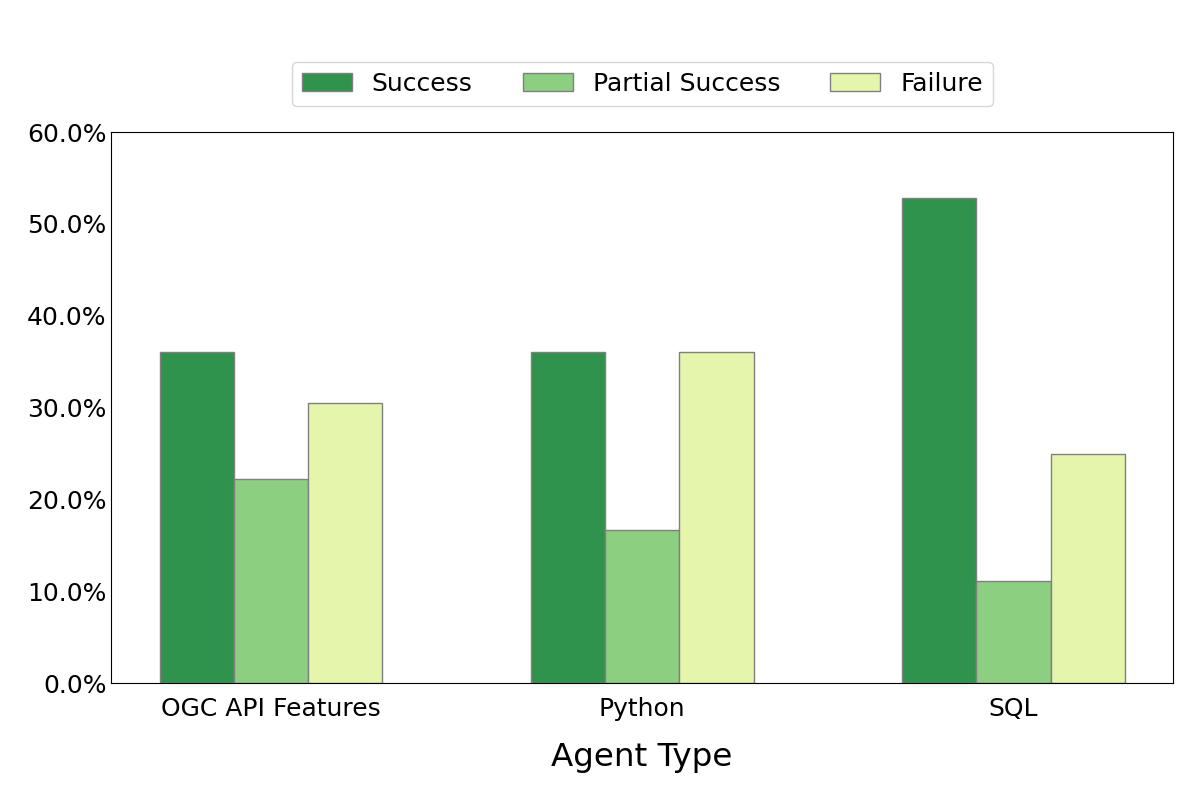
\includegraphics[width=\textwidth]{outcome_distribution_bar_chart.png}
    \caption{Outcome distribution between different agent types}
    \label{fig:outcome-distribution}
\end{figure}

From \autoref{fig:outcome-distribution}, we can read that the \acrshort{acr:ogc} \acrshort{acr:api} Features and Python agent have comparable results, and that the \acrshort{acr:sql}-based agent performs significantly better compared to the other two in terms of producing the desired outcome.

\subsubsection{Other Metrics}

\begin{figure}[htbp]
    \centering
    \begin{subfigure}[b]{0.48\textwidth}
        \centering
        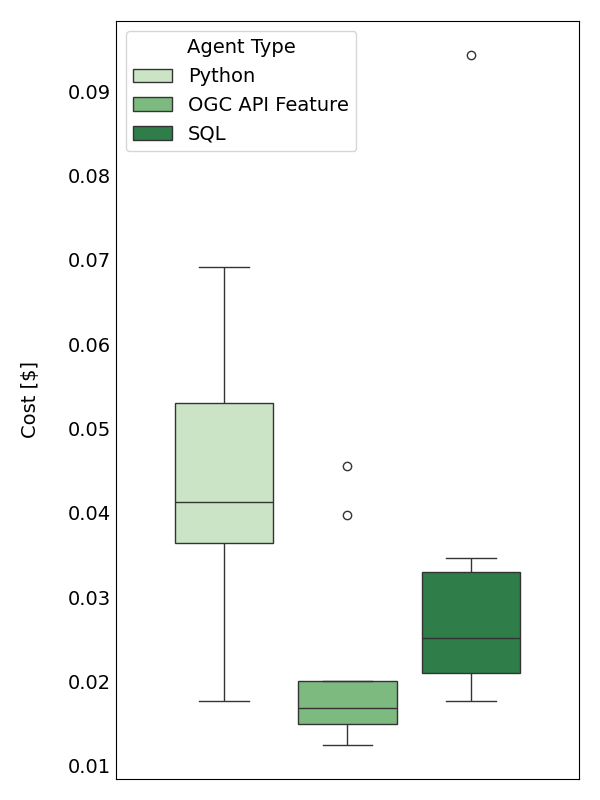
\includegraphics[width=\textwidth]{cost_box_plot.png}
        \caption{Average cost per call for each agent type}
        \label{fig:cost-box-plot}
    \end{subfigure}
    \hfill
    \begin{subfigure}[b]{0.48\textwidth}
        \centering
        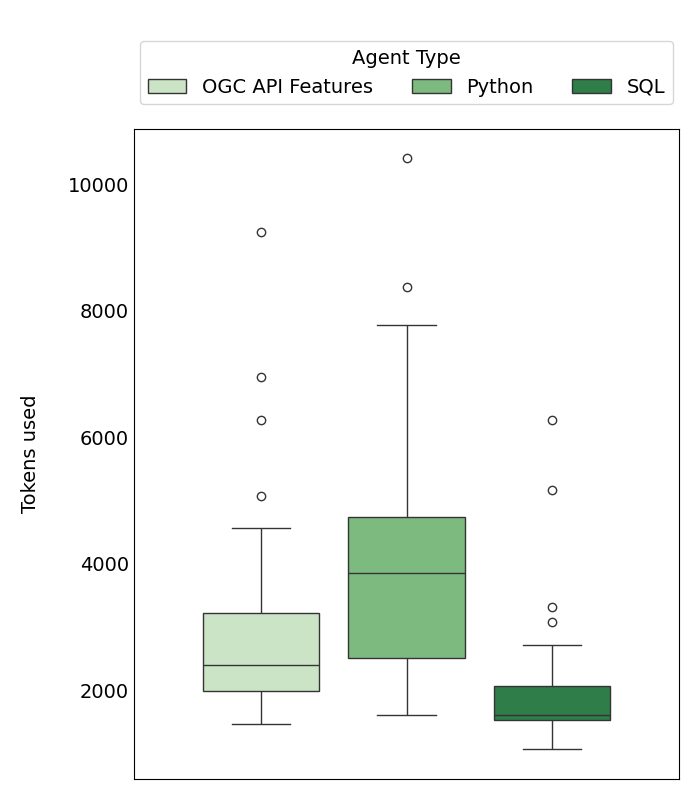
\includegraphics[width=\textwidth]{tokens_box_plot.png}
        \caption{Average token usage per agent type}
        \label{fig:tokens-box-plot}
    \end{subfigure}
    \caption{Cost and token usage}
    \label{fig:cost-and-tokens}
\end{figure}

\begin{figure}[htbp]
    \centering
    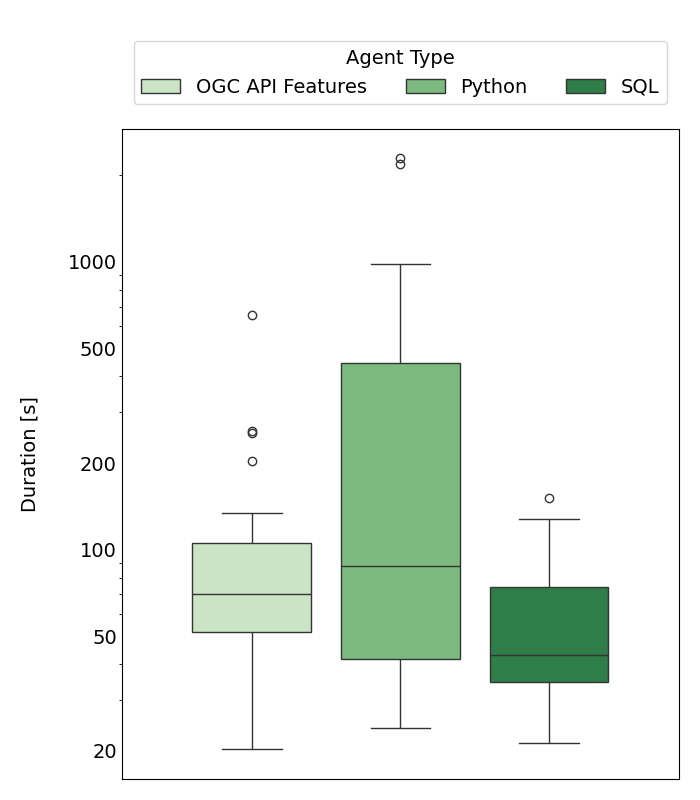
\includegraphics[width=0.6\textwidth]{duration_box_plot.png}
    \caption{Duration per Agent Type}
    \label{fig:duration-box-plot}
\end{figure}

\begin{figure}[htbp]
    \centering
    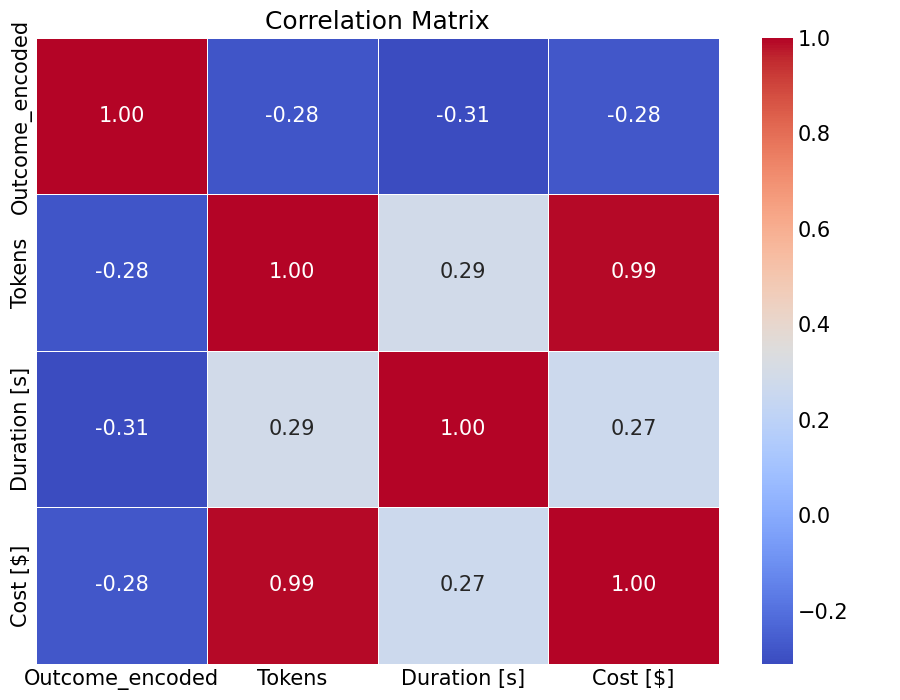
\includegraphics[width=0.7\textwidth]{correlation_matrix.png}
    \caption{Correlation matrix for test result metrics}
    \label{fig:correlation-matrix}
\end{figure}

\subsubsection{Repeatability}

\autoref{tbl:stddev-by-agent-type} shows the average standard deviation for each agent type, as well as the mean of these three standard deviations. The latter serves as an overall measure of GeoGPT's ability to repeatedly produce the desired outcome from a given query. Standard deviations were calculated for each triplet of identical test samples, in which both the question and the agent type remained the same. To produce a numerical value for the standard deviations, the encoded outcomes (see \autoref{tbl:outcome-encoding}) were used. Taking the average of the standard deviations for all 12 triplets for each agent type produced the numbers found in \autoref{tbl:stddev-by-agent-type}.

\begin{table}[htbp]
    \centering
    \caption{Standard Deviation by Agent Type}
    \label{tbl:stddev-by-agent-type}
    \begin{tabularx}{0.7\textwidth}{XX}
        \toprule
        \textbf{Agent Type} & \textbf{Outcome Std. Deviation} \\
        \midrule
        OGC API Features    & 0.552                           \\
        Python              & 0.337                           \\
        SQL                 & 0.337                           \\
        \midrule
        \textbf{Mean}       & 0.408                           \\
        \bottomrule
    \end{tabularx}
\end{table}

\subsection{Prompt Quality Test Results}
\label{subsec:prompt-quality-test-results}

\begin{figure}[htbp]
    \centering
    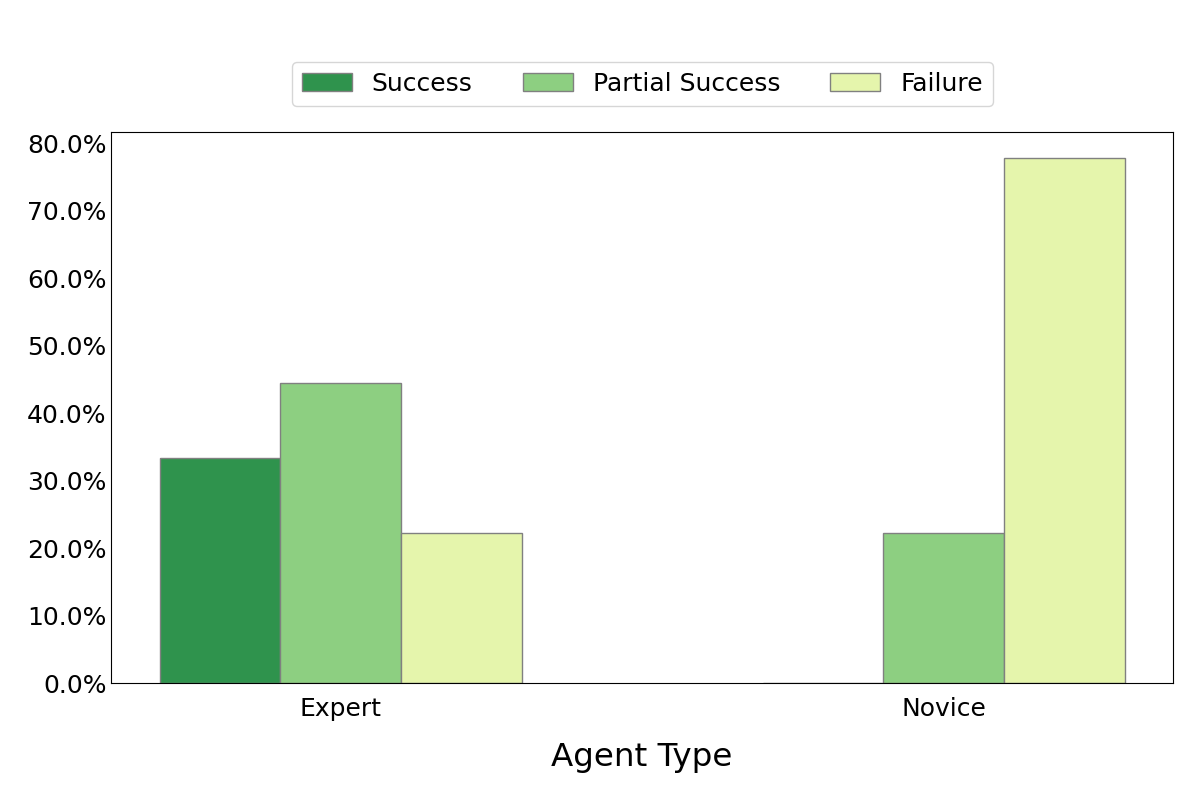
\includegraphics[width=\textwidth]{levels_outcome_distribution_bar_chart.png}
    \caption{Outcome distribution for different levels of GIS experience}
    \label{fig:outcome-distribution-experience-levels}
\end{figure}

\autoref{fig:novice-vs-expert-munkegata-trees} shows a comparison between the results GeoGPT managed to produce for two different prompts that one would expect to produce identical outcomes. The \textit{novice}-level prompt was as follows:

\begin{quote}
    \enquote{Could you count how many trees there are on Munkegata street in Trondheim?}
\end{quote}

\noindent The \textit{expert}-level prompt, on the other hand, included a series of instructions:

\begin{quote}
    \enquote{1. List all datasets that could possibly include trees. \\
        2. Find the correct feature class and filter the relevant dataset to access tree data for Trondheim. Use a bounding box to reduce the number of trees to analyse. \\
        4. Fetch road data for Munkegata. Use a bounding box for Trondheim in case there are streets elsewhere named Munkegata. \\
        5. Convert both datasets to a suitable metric CRS and add a 20-meter buffer around the road data. \\
        6. Find all trees that lie within this buffer and count them. \\
        7. Present the findings with a map highlighting the roads and the trees.}
\end{quote}

Using novice-level prompt GeoGPT was unable to produce the correct outcome, and confidently answered that there are \enquote{approximately 6,915 trees on Munkegata street in Trondheim.}, which is far from being true. When solving the task, GeoGPT made a series of oversights that lead to this result. First, GeoGPT failed to take into account that there may be more than one street in the dataset with the name \enquote{Munkegata}, \enquote{forgetting} to use a bounding box when retrieving the road data from the \acrshort{acr:api}. The same mistake was made when retrieving the tree data. Due to the upper limit of 10,000 features per query in the \acrshort{acr:api}, it's crucial to narrow down the query to ensure retrieval of all relevant features rather than just a subset. GeoGPT's query for tree data lacked a bounding box, resulting in a randomly distributed subset scattered across Norway. A third mistake occurred when GeoGPT calculated a bounding box around the retrieved road data instead of creating a buffer. The latter method would have produced a more accurate result. The bounding box that was created spanned from Trondheim to Oslo, thus including far more trees than was intended.



\begin{figure}[htbp]
    \centering
    \begin{subfigure}[b]{0.48\textwidth}
        \centering
        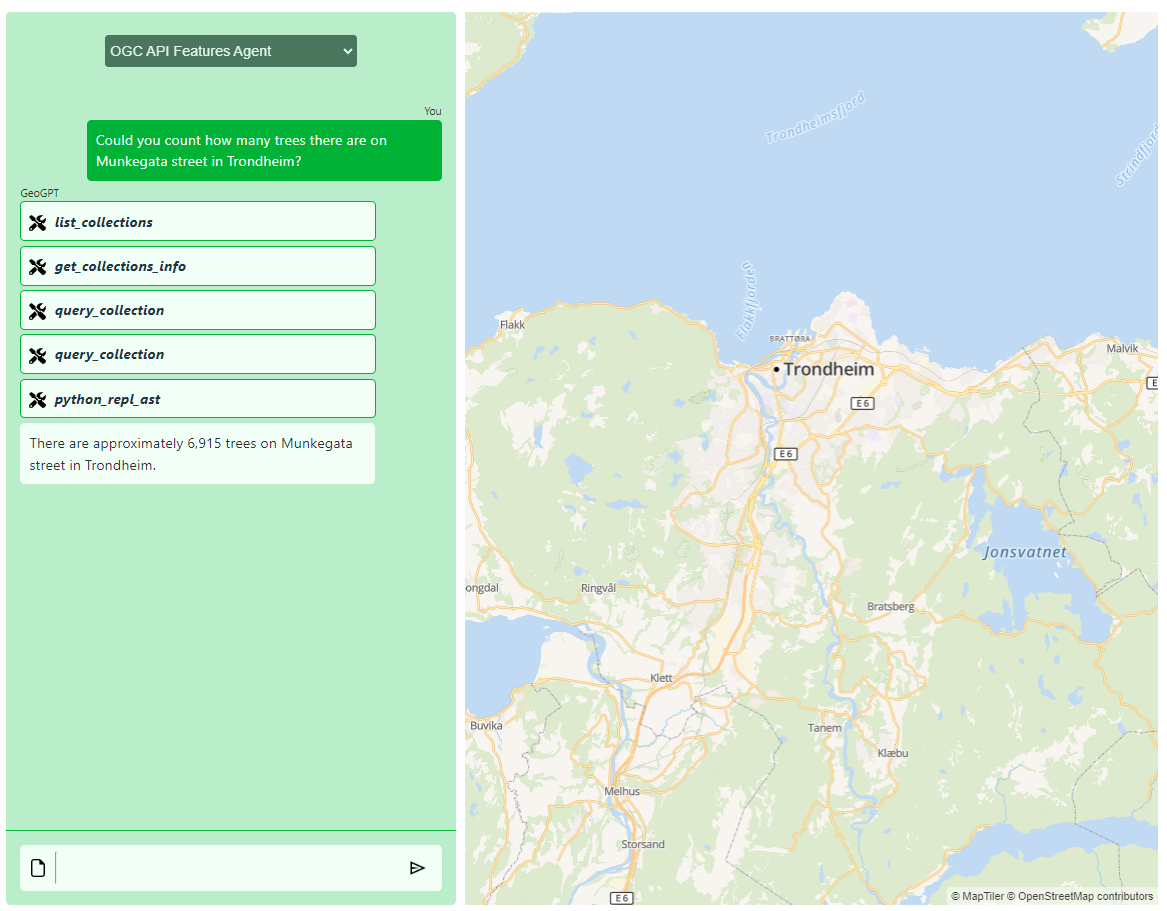
\includegraphics[width=\textwidth]{munkegata_trees_oaf_novice.png}
        \caption{Novice-level prompting}
        \label{fig:novice-level-prompting-munkegata-trees}
    \end{subfigure}
    \hfill
    \begin{subfigure}[b]{0.48\textwidth}
        \centering
        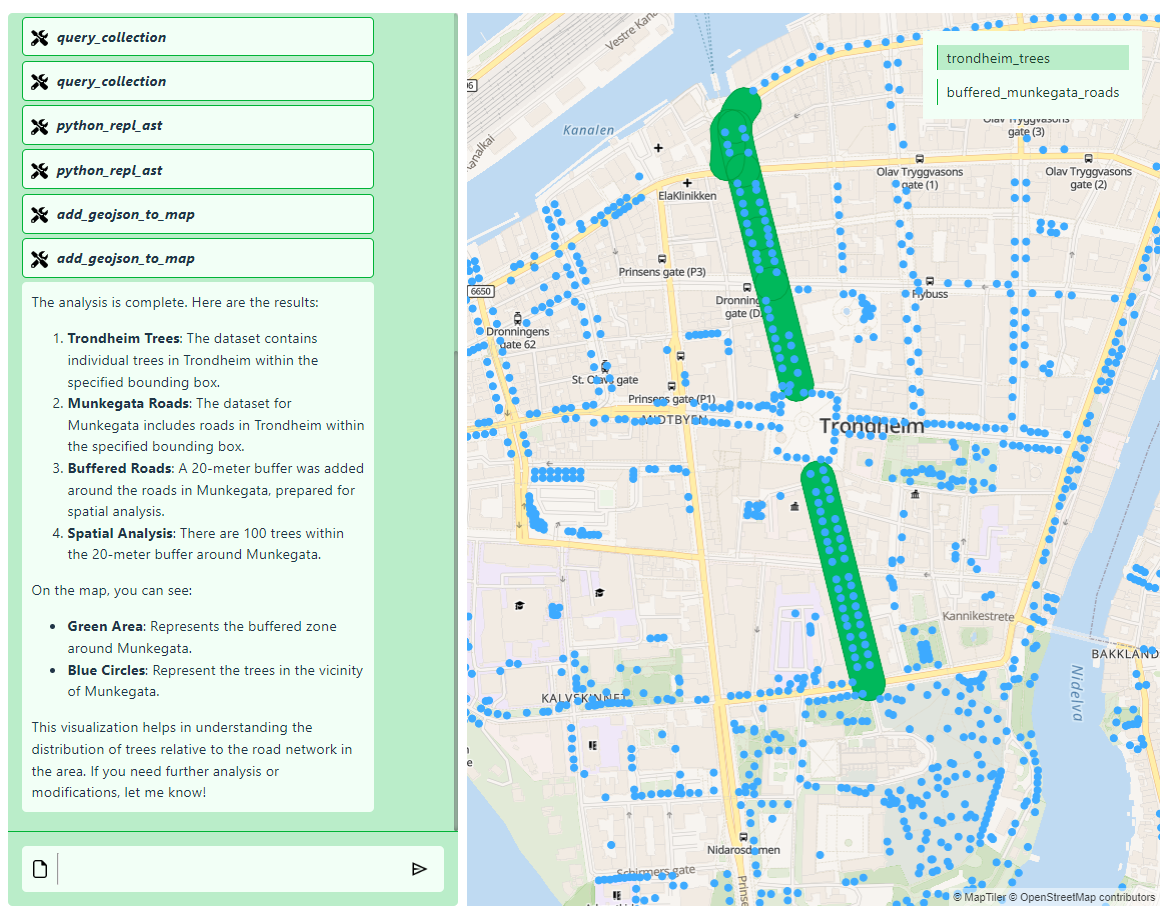
\includegraphics[width=\textwidth]{munkegata_trees_oaf_expert_sbs_2.png}
        \caption{Expert-level prompting}
        \label{fig:expert-level-prompting-munkegata-trees}
    \end{subfigure}
    \caption{Comparison between novice and expert level prompting for making GeoGPT's \acrshort{acr:ogc} \acrshort{acr:api} Features agent calculate the number of trees along Munkegata in Trondheim}
    \label{fig:novice-vs-expert-munkegata-trees}
\end{figure}


